Riak is available in two versions. There is Riak TS for Time Series Data and Riak KV. The chapter about Riak concentrates on Riak KV (further "Riak").
\section{Introducion into Riak}
The following chapter will give you an introduction into Riak and its main features. 
\subsection{General Information}
Riak is a distributed key-value NoSQL database which is designed for high availability. As long as the client can reach one Riak server the data is available since data is saved across multiple servers. How the clustering works will be shown in the next chapter. 
\\
Riak is available for different operating systems, e.g. Ubuntu, CentOS or Mac OS X but not for Windows. The installation is straight-forward because you just have to download a package from the official website and install the package. 
\\ 
As data is saved across multiple servers even hardware or network failures can be handled by Riak. If you need more space for your data new servers can be added easily. By adding new servers the scalability is nearly linear which is very impressive. 
\\
Data is saved in buckets. A bucket in Riak can be compared with a table in a SQL-database. 
\\ 
Now if you have a look on the CAP-Theorem one can say that Riak definitely concentrates on "A" and "P" - Availability and Partition Tolerance. If your system needs a high availability and you can't accept downtime Riak is probably the best solution. Another feature of Riak is its latency: since the CRUD-operations don't involve complex joins the requests are serviced promptly.
\\
On the other hand if your system needs a high consistency of the data Riak is not the right choice. 
\subsection{Riak Clustering}
The high availability of Riak can only be achieved by the Riak clustering. The official website of Riak recommends that there should be at least 5 nodes in one cluster. A node is a server in production environment - during the development of the software there can be more than one node on a server. 
\\
All nodes have the same responsibility, so there is no kind of master-node which has special tasks. 

The clustering is visible in the logo of Riak, too. There is one node and three lines to three other nodes which symbolizes the replication of data:
\begin{figure}[h!]
	\centering
	
\includegraphics[width=3.0in]{riak_logo.png}
	\caption{Riak Logo}
	\label{Riak Logo}
\end{figure}

\subsubsection{Automatic re-distribution of data}
When new servers are added or when machines are removed  Riak automatically re-distributes the data with no downtime. Data is spread in the cluster until each node owns the same amount of data. So developers don't need to care about where the data is saved. Riak uses consistent hashing to distribute data evenly across the nodes in a cluster. Consistent hashing limits the reshuffling of keys when a hash-table structure is rebalanced.
\subsubsection{Intelligent Replication}
Even if nodes go down the user should be able to read and write data. The replication scheme ensures this by setting a replication variable, that specifies the number of nodes on which a value will be replicated. The default number is 3 which means that each object is replicated 3 times. If Riak can access one node there the object is replicated it's available for the client.
\\ 
The following picture describes the replication: 
\begin{figure}[h]
	\centering
	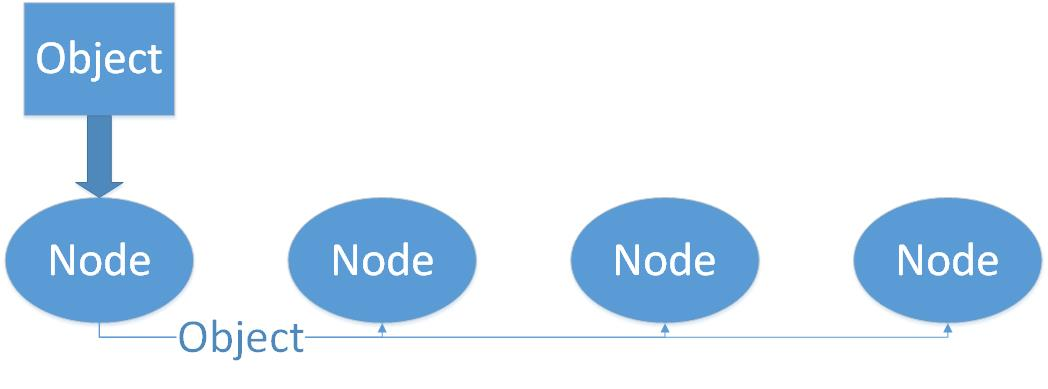
\includegraphics[width=3.0in]{riak_clustering.jpg}
	\caption{Riak Clustering}
	\label{Riak Clustering}
\end{figure}